 \documentclass[11pt]{article} 
\usepackage[english]{babel}
\usepackage[utf8]{inputenc}
\usepackage[margin=0.5in]{geometry}
\usepackage{amsmath}
\usepackage{amsthm}
\usepackage{amsfonts}
\usepackage{amssymb}
\usepackage[usenames,dvipsnames]{xcolor}
\usepackage{graphicx}
\usepackage[siunitx]{circuitikz}
\usepackage{tikz}
\usepackage{tkz-berge}
\usetikzlibrary{positioning, automata, backgrounds}
\usepackage[colorinlistoftodos, color=orange!50]{todonotes}
\usepackage{hyperref}
\usepackage[numbers, square]{natbib}
\usepackage{fancybox}
\usepackage{epsfig}
\usepackage{soul}
\usepackage[framemethod=tikz]{mdframed}
\usepackage[shortlabels]{enumitem}
\usepackage[version=4]{mhchem}
\usepackage{multicol}
\usepackage{forest}
\usepackage{mathtools}
\usepackage{comment}
\usepackage{enumitem}
\usepackage[utf8]{inputenc}
\usepackage{listings}
\usepackage{color}
\usepackage[numbers]{natbib}
\usepackage{subfiles}
\usepackage{tkz-berge}
\usepackage{algorithm}
\usepackage[noend]{algpseudocode}


\newtheorem{prop}{Proposition}[section]
\newtheorem{thm}{Theorem}[section]
\newtheorem{lemma}{Lemma}[section]
\newtheorem{cor}{Corollary}[prop]

\theoremstyle{definition}
\newtheorem{definition}{Definition}

\theoremstyle{definition}
\newtheorem{required}{Problem}

\theoremstyle{definition}
\newtheorem{ex}{Example}

\newcommand{\interval}[4]{\draw (#2, #1) -- (#3, #1); % Usage: \interval{height}{start}{end}{label}
\draw (#2, #1-0.11) -- (#2, #1+0.11); % draw left whisker
\draw (#3, #1-0.11) -- (#3, #1+0.11); % draw right whisker
\node[] at (#2-0.25, #1) {#4};
}


\setlength{\marginparwidth}{3.4cm}
%#########################################################

%To use symbols for footnotes
\renewcommand*{\thefootnote}{\fnsymbol{footnote}}
%To change footnotes back to numbers uncomment the following line
%\renewcommand*{\thefootnote}{\arabic{footnote}}

% Enable this command to adjust line spacing for inline math equations.
% \everymath{\displaystyle}

% _______ _____ _______ _      ______ 
%|__   __|_   _|__   __| |    |  ____|
%   | |    | |    | |  | |    | |__   
%   | |    | |    | |  | |    |  __|  
%   | |   _| |_   | |  | |____| |____ 
%   |_|  |_____|  |_|  |______|______|
%%%%%%%%%%%%%%%%%%%%%%%%%%%%%%%%%%%%%%%

\title{
\normalfont \normalsize 
\textsc{CSCI 3104 Spring 2022 \\ 
Instructors: Profs. Chen and Layer} \\
[10pt] 
\rule{\linewidth}{0.5pt} \\[6pt] 
\huge Problem Set 8 \\
\rule{\linewidth}{2pt}  \\[10pt]
}
%\author{Your Name}
\date{}

\begin{document}
\definecolor {processblue}{cmyk}{0.96,0,0,0}
\maketitle


%%%%%%%%%%%%%%%%%%%%%%%%%
%%%%%%%%%%%%%%%%%%%%%%%%%%
%%%%%%%%%%FILL IN YOUR NAME%%%%%%%
%%%%%%%%%%AND STUDENT ID%%%%%%%%
%%%%%%%%%%%%%%%%%%%%%%%%%%
\noindent
Due Date \dotfill March 29 \\
Name \dotfill \textbf{Chengming Li} \\
Student ID \dotfill \textbf{109251991} \\
Collaborators \dotfill \textbf{N/A}

\tableofcontents

\section{Instructions}
 \begin{itemize}
	\item The solutions \textbf{must be typed}, using proper mathematical notation. We cannot accept hand-written solutions. \href{http://ece.uprm.edu/~caceros/latex/introduction.pdf}{Here's a short intro to \LaTeX.}
	\item You should submit your work through the \textbf{class Canvas page} only. Please submit one PDF file, compiled using this \LaTeX \ template.
	\item You may not need a full page for your solutions; pagebreaks are there to help Gradescope automatically find where each problem is. Even if you do not attempt every problem, please submit this document with no fewer pages than the blank template (or Gradescope has issues with it).

	\item You are welcome and encouraged to collaborate with your classmates, as well as consult outside resources. You must \textbf{cite your sources in this document.} \textbf{Copying from any source is an Honor Code violation. Furthermore, all submissions must be in your own words and reflect your understanding of the material.} If there is any confusion about this policy, it is your responsibility to clarify before the due date. 

	\item Posting to \textbf{any} service including, but not limited to Chegg, Reddit, StackExchange, etc., for help on an assignment is a violation of the Honor Code.
\end{itemize}

\newpage
\section{Standard 22 - Dynamic Programming: Bactracking to Find Solutions}
\begin{required}
Consider the following input for the Knapsack problem with a capacity $W=11$:\\
\begin{center}
 \begin{tabular}{r|c|c|c|c|c|c}
        item $i$  & 1  & 2 &3 &4 &5 &6 \\
                \hline
        value $v_i$ &2 & 6& 19&24 &29 &34 \\
          \hline
        weight $w_i$ & 1 & 2  & 5& 6& 7& 8\\
                 \end{tabular}
\end{center}

\vspace{1mm}
\noindent \\ 
and the corresponding table for the optimal values/profits:\\
\begin{center}
 \begin{tabular}{r|c|c|c|c|c|c|c|c|c|c|c|c}
          & 0  & 1 &2 &3 &4&5&6&7&8&9&10&11 \\
                \hline
        \{  \}  &0 & 0& 0&0 &0 &0&0 & 0& 0&0 &0 &0 \\
          \hline
         \{ 1 \}  & 0 & 2  & 2& 2& 2& 2& 2  & 2& 2& 2& 2&2\\
          \hline
           \{1,~2  \}  & 0 & 2  & 6& 8& 8& 8& 8& 8& 8& 8& 8& 8\\
          \hline
           \{ 1,~2,~3 \}  & 0 & 2  & 6&8& 8& 19&21&25&27&27&27&27\\
          \hline
           \{1,~2,~3,~4  \}  & 0 & 2  & 6& 8& 8& 19&24&26&30&32&32&43\\
          \hline
           \{1,~2,~3,~4,~5  \}  & 0 & 2  & 6& 8& 8& 19&24&29&31&35&37&43\\
          \hline
           \{ 1,~2,~3,~4,~5,~6 \}  & 0 & 2  & 6& 8& 8& 19&24&29&34&36&40&43\\
          
          
                 \end{tabular}
\end{center}

\vspace{1mm}
\noindent \\ 
Draw the backward path consisting of backward edges to find the subset of items that has the optimal value/profit. Besides indicating the backward path, you must also give the optimal-value subset of items.
Clearly explain your work. 

\begin{proof}[Answer]
%Your answer here
\begin{align*}
OPT(i,w) = \begin{cases}
0  &  i = 0\\
OPT(i-1,w) &  w_i > w \\
max\{OPT(i-1,w),v_i+OPT(i-1,w-w_i)\} &  otherwise\\
\end{cases}
\end{align*}

\begin{itemize}
\item For item 6:\\
\\OPT(6,11) = 43, we choose third condition because $w_6 = 8 < 11$. And in this condition,we have $max\{OPT(5,11) = 43 ,34+OPT(5,3)= 34+8=42\}$. So \textbf{we choose OPT(5,11) = 43}\\
OPT(5,11) = 43, we choose third condition because $w_5 = 7 < 11$. And in this condition,we have $max\{OPT(4,11) = 43 ,24+OPT(4,4)= 29+8=37\}$. So \textbf{we choose OPT(4,11) = 43}\\
OPT(4,11) = 43, we choose third condition because $w_4 = 6 < 11$. And in this condition,we have $max\{OPT(3,11) = 27 ,19+OPT(3,5)= 24+19=43\}$. So \textbf{we choose $w_4 + OPT(3,5) = 24+19$}.\\
OPT(3,5) = 19, we choose third condition because $w_3 = 5 = 5$. And in this condition,we have $max\{OPT(2,5) = 8 ,19+OPT(2,0)= 19+0=19\}$. So \textbf{we choose $w_3 + OPT(2,0) = 24+19$}.\\
OPT(2,0) = 0, we choose second condition because $w_2 = 2 > 0$. And in this condition,we have OPT(1,0) = 0. So \textbf{we choose  OPT(1,0) = 0}.\\
OPT(1,0) = 0, we choose second condition because $w_1 = 1 > 0$. And in this condition,we have OPT(0,0) = 0. So \textbf{we choose  OPT(0,0) = 0}.\\
\textbf{The path is OPT(6,11) -$>$ OPT(5,11) -$>$ OPT(4,11) -$>$ OPT(3,5) -$>$ OPT(2,0) -$>$ OPT(1,0) -$>$ OPT(0,0)}


\item For item 5:\\
OPT(5,11) = 43, we choose third condition because $w_5 = 7 < 11$. And in this condition,we have $max\{OPT(4,11) = 43 ,24+OPT(4,4)= 29+8=37\}$. So \textbf{we choose OPT(4,11) = 43}\\
OPT(4,11) = 43, we choose third condition because $w_4 = 6 < 11$. And in this condition,we have $max\{OPT(3,11) = 27 ,19+OPT(3,5)= 24+19=43\}$. So \textbf{we choose $w_4 + OPT(3,5) = 24+19$}.\\
OPT(3,5) = 19, we choose third condition because $w_3 = 5 = 5$. And in this condition,we have $max\{OPT(2,5) = 8 ,19+OPT(2,0)= 19+0=19\}$. So \textbf{we choose $w_3 + OPT(2,0) = 24+19$}.\\
OPT(2,0) = 0, we choose second condition because $w_2 = 2 > 0$. And in this condition,we have OPT(1,0) = 0. So \textbf{we choose  OPT(1,0) = 0}.\\
OPT(1,0) = 0, we choose second condition because $w_1 = 1 > 0$. And in this condition,we have OPT(0,0) = 0. So \textbf{we choose  OPT(0,0) = 0}.\\
\textbf{The path is  OPT(5,11) -$>$ OPT(4,11) -$>$ OPT(3,5) -$>$ OPT(2,0) -$>$ OPT(1,0) -$>$ OPT(0,0)}

\item For item 4:\\
OPT(4,11) = 43, we choose third condition because $w_4 = 6 < 11$. And in this condition,we have $max\{OPT(3,11) = 27 ,19+OPT(3,5)= 24+19=43\}$. So \textbf{we choose $w_4 + OPT(3,5) = 24+19$}.\\
OPT(3,5) = 19, we choose third condition because $w_3 = 5 = 5$. And in this condition,we have $max\{OPT(2,5) = 8 ,19+OPT(2,0)= 19+0=19\}$. So \textbf{we choose $w_3 + OPT(2,0) = 24+19$}.\\
OPT(2,0) = 0, we choose second condition because $w_2 = 2 > 0$. And in this condition,we have OPT(1,0) = 0. So \textbf{we choose  OPT(1,0) = 0}.\\
OPT(1,0) = 0, we choose second condition because $w_1 = 1 > 0$. And in this condition,we have OPT(0,0) = 0. So \textbf{we choose  OPT(0,0) = 0}.\\
\textbf{The path is  OPT(4,11) -$>$ OPT(3,5) -$>$ OPT(2,0) -$>$ OPT(1,0) -$>$ OPT(0,0)}

\item For item 3:\\
OPT(3,8) = 27, we choose third condition because $w_3 = 5 < 8$. And in this condition,we have $max\{OPT(2,8) = 27 ,19+OPT(2,3)= 19+8=27\}$. So \textbf{we choose $w_3 + OPT(2,3) = 19+8$}.\\
OPT(2,3) = 8, we choose third condition because $w_2= 2 < 3$. And in this condition,we have $max\{OPT(1,3) = 2 ,6+OPT(1,1)= 6+2=8\}$. So \textbf{we choose $w_2 + OPT(1,1) = 6+2$}.\\
OPT(1,1) = 2, we choose third condition because $w_1= 1 = 1$. And in this condition,we have $max\{OPT(0,1) = 0 ,2+OPT(0,0)= 2+0=2\}$. So \textbf{we choose  2+OPT(0,0)= 2+0}.\\
\textbf{The path is  OPT(3,8) -$>$ OPT(2,3) -$>$ OPT(1,1) -$>$ OPT(0,0) }

\item For item 2:\\
OPT(2,3) = 8, we choose third condition because $w_2= 2 < 3$. And in this condition,we have $max\{OPT(1,3) = 2 ,6+OPT(1,1)= 6+2=8\}$. So \textbf{we choose $w_2 + OPT(1,1) = 6+2$}.\\
OPT(1,1) = 2, we choose third condition because $w_1= 1 = 1$. And in this condition,we have $max\{OPT(0,1) = 0 ,2+OPT(0,0)= 2+0=2\}$. So \textbf{we choose  2+OPT(0,0)= 2+0}.\\
\textbf{The path is OPT(2,3) -$>$ OPT(1,1) -$>$ OPT(0,0) }

\item For item 1:\\
OPT(1,1) = 2, we choose third condition because $w_1= 1 = 1$. And in this condition,we have $max\{OPT(0,1) = 0 ,2+OPT(0,0)= 2+0=2\}$. So \textbf{we choose  2+OPT(0,0)= 2+0}.\\
\textbf{The path is OPT(1,1) -$>$ OPT(0,0) }

\end{itemize}
\end{proof}


\end{required}


\newpage
\begin{required}
Recall the sequence alignment problem where the cost of {\em sub} and the cost of {\em indel} are all $1$. Given the following table of optimal cost of aligning the strings EXPONEN and POLYNO, draw the backward path consisting of backward edges to find the minimal-cost set of edit operations that transforms EXPONEN to POLYNO. Besides indicating the backward path, you must also give the minimal-cost set of edit operations.  Clearly explain your work. 
 % ----- FIGURE -----
        \begin{figure}[h!]
        \begin{center}
        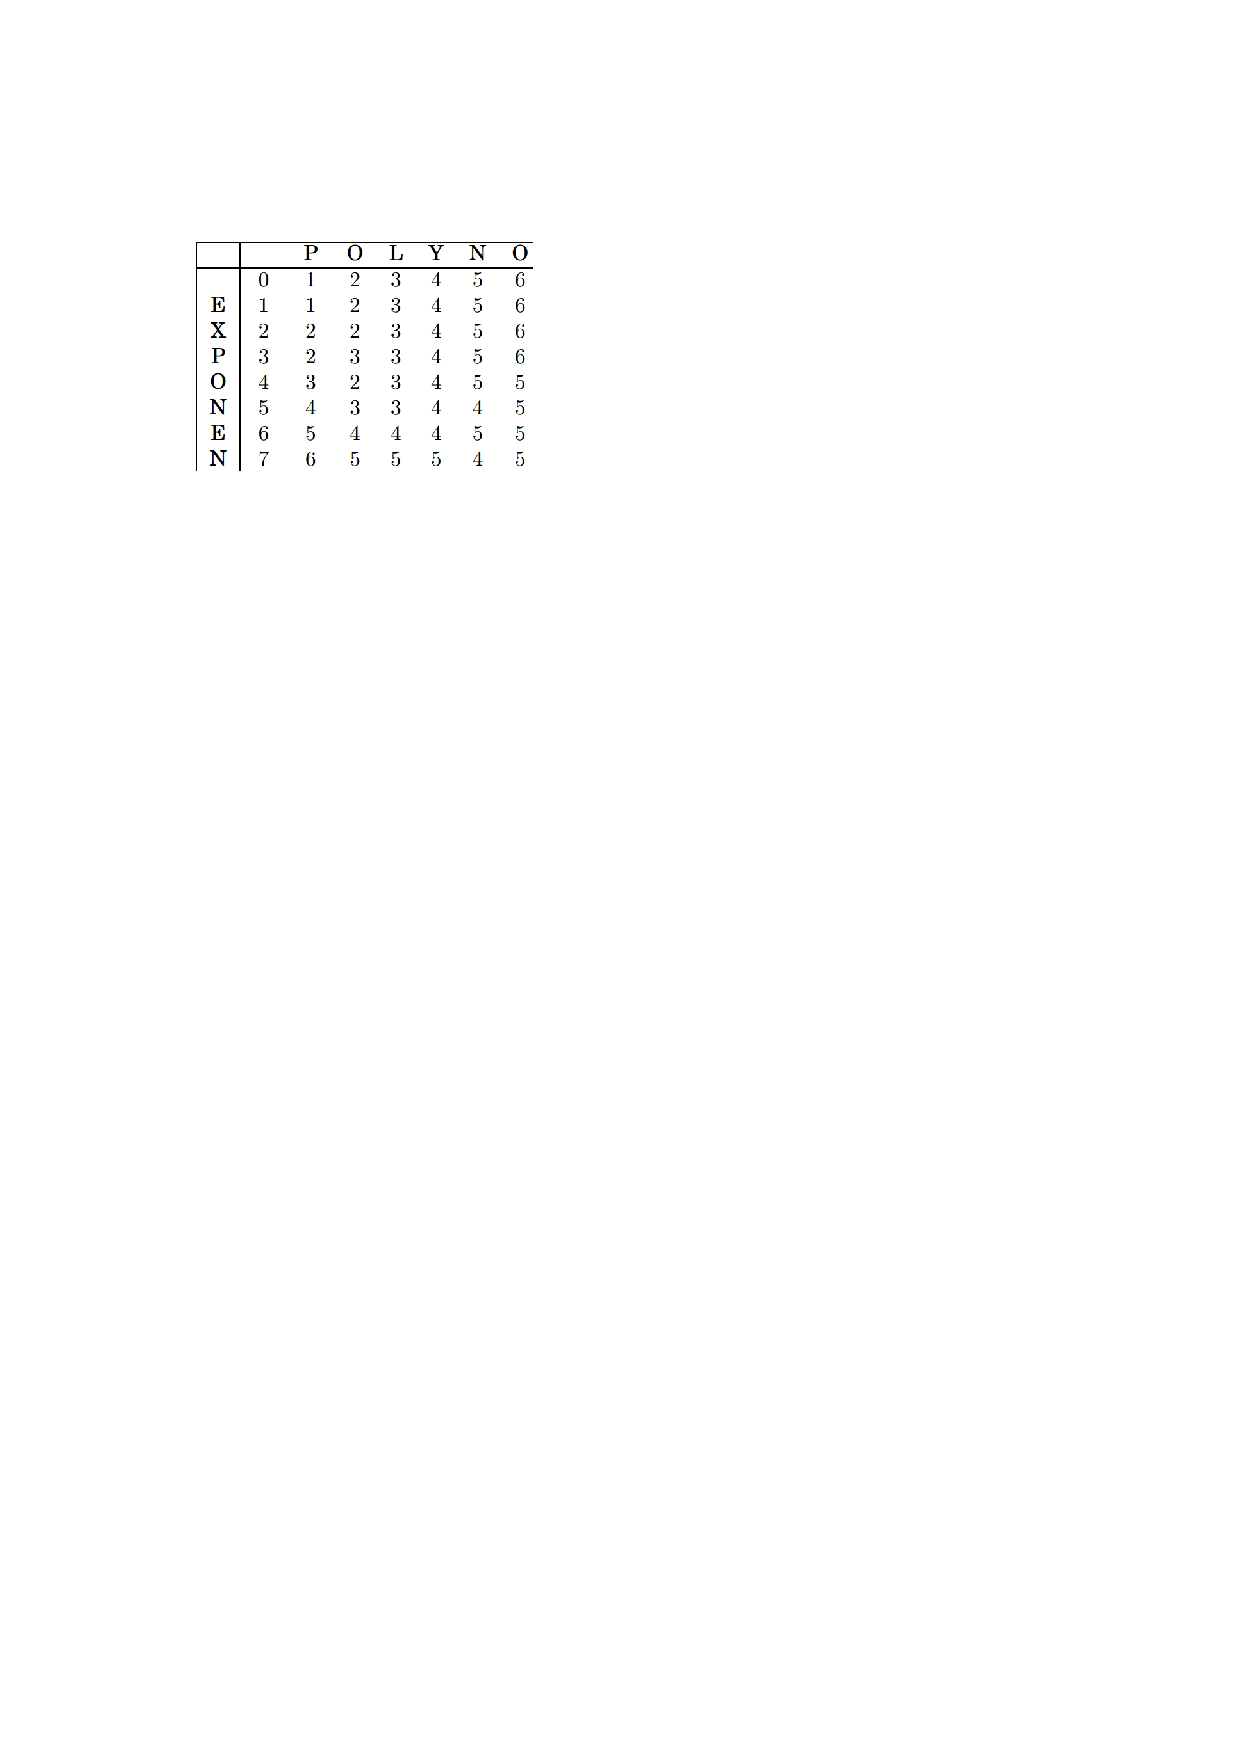
\includegraphics[scale=0.90]{exp_poly.pdf} 
        \end{center}
        \end{figure}
        % ----------

\begin{proof}[Answer]
%Your answer here
\begin{center}
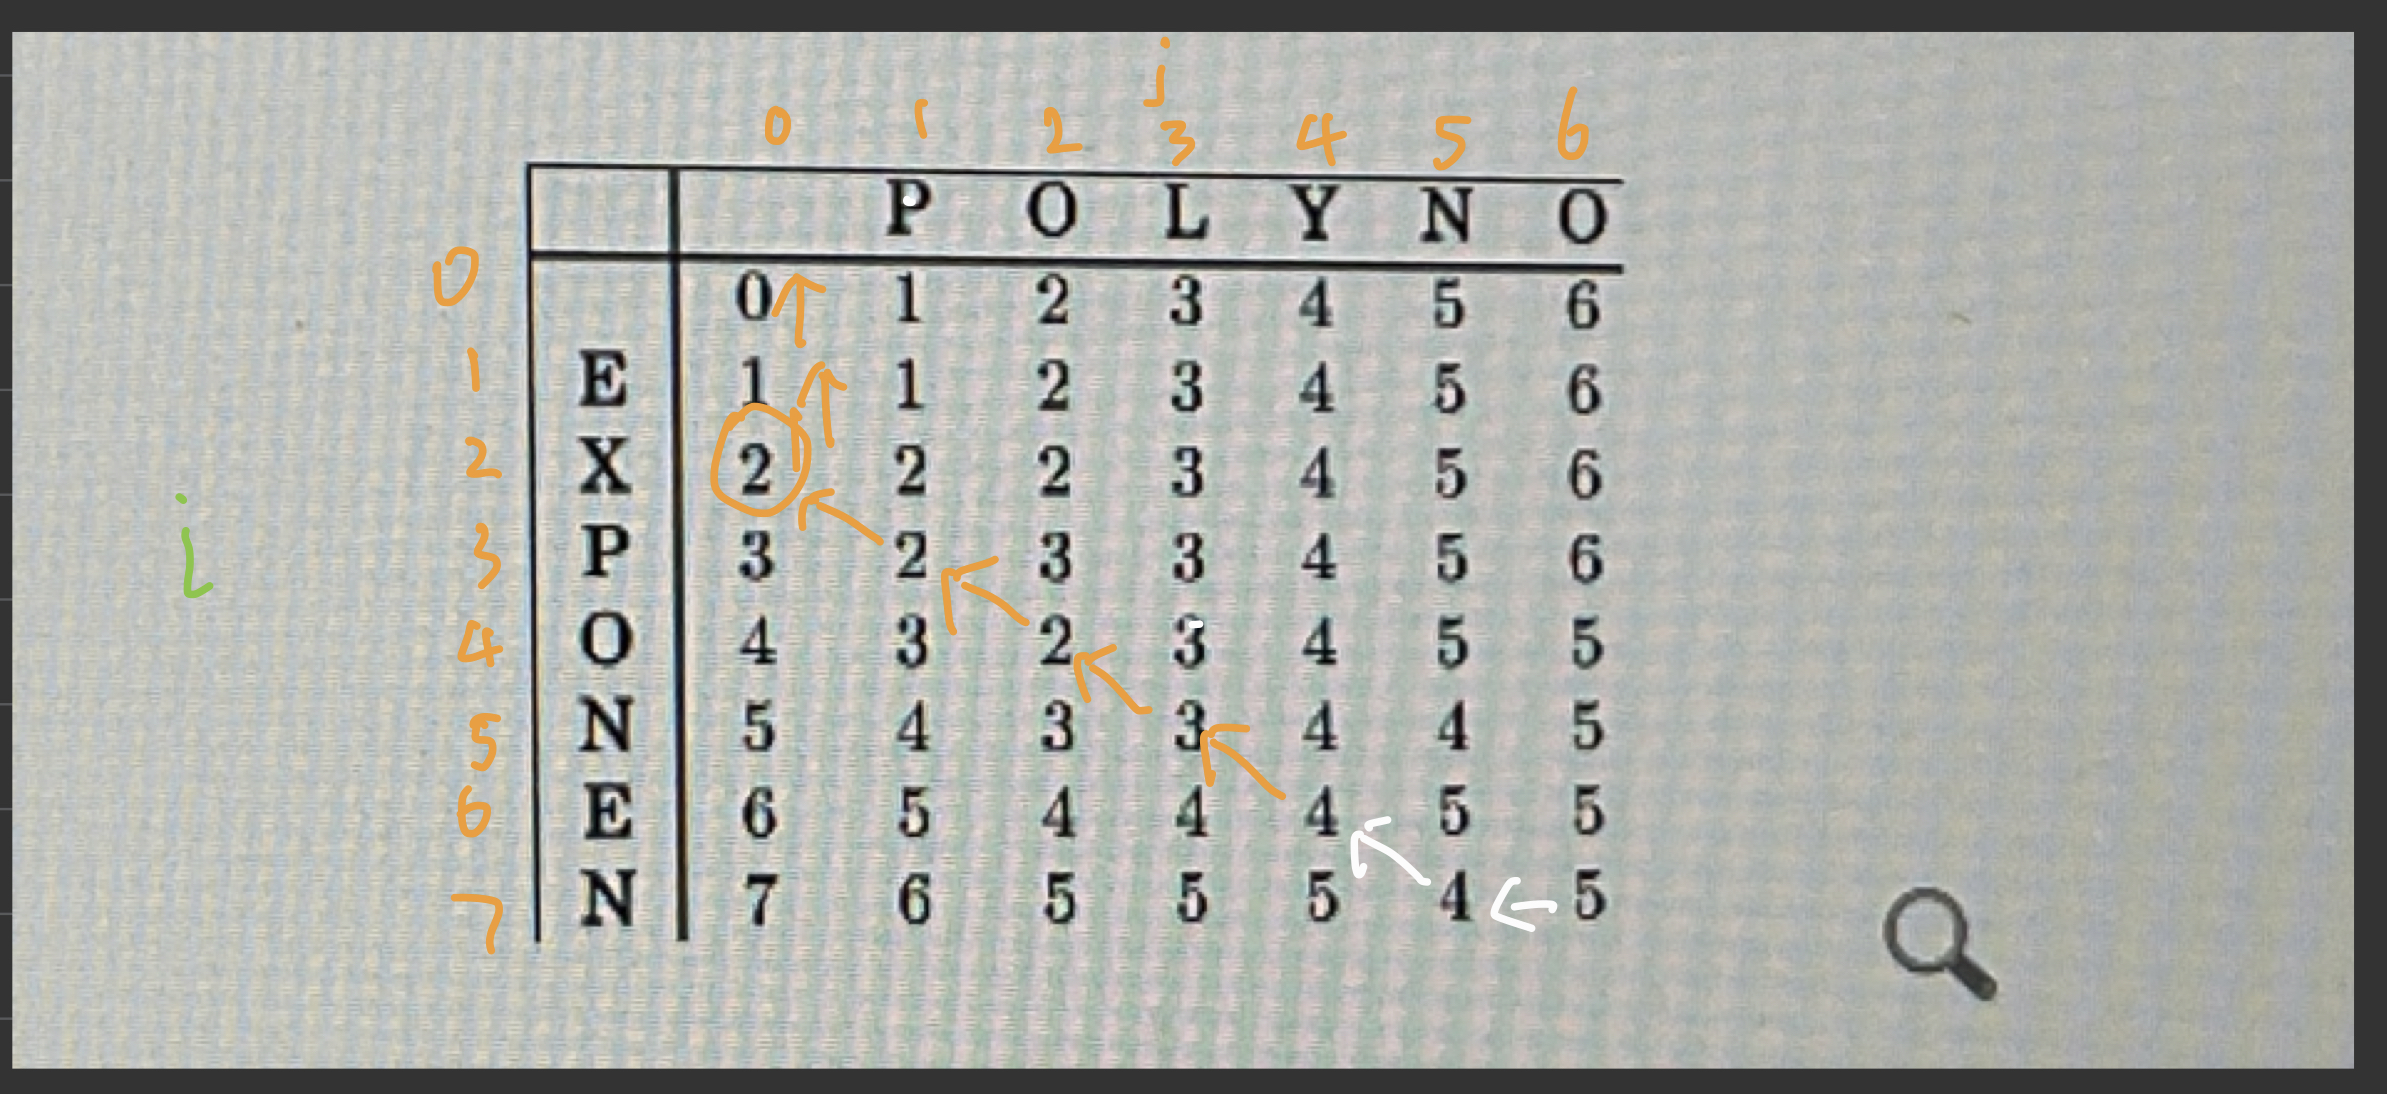
\includegraphics[width=0.7\textwidth]{IMG_0509.PNG}
\end{center}
\begin{align*}
cost(i,j) = min\begin{cases}
cost(i-1,j-1) + c(sub) \\
cost(i-1,j) + c(indel) \\
cost(i,j-1) + c(indel)\\
cost(i-1,j-1) & if (x_i = y_j)
\end{cases}
\end{align*}

\textbf{The path is $cost(7,6) -> cost(7,5) -> cost(6,4) -> cost(5,3) -> cost(4,2) -> cost(3,1) ->cost(2,0) -> cost(1,0) ->cost(0,0)$}\\
\\\textbf{cost(7,6) = cost(7,5)+1(indel) = 5 because it is the minimum cost and $x_i \neq y_j$}\\
\begin{align*}
cost(7,6) = min\begin{cases}
cost(6,5) + c(sub) = 6 \\
cost(6,6) + c(indel) = 6\\
cost(7,5) + c(indel) = 5\\
cost(6,5) = 5 & if (x_i = y_j)
\end{cases}
\end{align*}
\newpage
\textbf{cost(7,5) = cost(6,4)+0(sub) = 4 because it is the minimum cost and$ x_i = y_j$}\\
\begin{align*}
cost(7,5) = min\begin{cases}
cost(6,4) + c(sub) = 5 \\
cost(6,5) + c(indel) = 6\\
cost(7,4) + c(indel) = 6\\
cost(6,4) = 4 & if (x_i = y_j)
\end{cases}
\end{align*}

\textbf{cost(6,4) = cost(5,3)+1(sub) = 4 because it is the minimum cost and$ x_i \neq y_j$}\\
\begin{align*}
cost(6,4) = min\begin{cases}
cost(5,3) + c(sub) = 4 \\
cost(5,4) + c(indel) = 5\\
cost(6,3) + c(indel) = 5\\
cost(5,3) = 3 & if (x_i = y_j)
\end{cases}
\end{align*}

\textbf{cost(5,3) = cost(4,2)+1(sub) = 3 because it is the minimum cost and$ x_i \neq y_j$}\\
\begin{align*}
cost(5,3) = min\begin{cases}
cost(4,2) + c(sub) = 3 \\
cost(4,3) + c(indel) = 4\\
cost(5,2) + c(indel) = 4\\
cost(4,2) = 2 & if (x_i = y_j)
\end{cases}
\end{align*}

\textbf{cost(4,2) = cost(3,1)+0(sub) = 2 because it is the minimum cost and$ x_i = y_j$}\\
\begin{align*}
cost(4,2) = min\begin{cases}
cost(3,1) + c(sub) = 3 \\
cost(3,2) + c(indel) = 4\\
cost(4,1) + c(indel) = 4\\
cost(3,1) = 2 & if (x_i = y_j)
\end{cases}
\end{align*}

\textbf{cost(3,1) = cost(2,0)+0(sub) = 2 because it is the minimum cost and$ x_i = y_j$}\\
\begin{align*}
cost(3,1) = min\begin{cases}
cost(2,0) + c(sub) = 3 \\
cost(2,1) + c(indel) = 3\\
cost(3,0) + c(indel) = 4\\
cost(2,0) = 2 & if (x_i = y_j)
\end{cases}
\end{align*}

\textbf{cost(2,0) = cost(1,0)+1(indel) = 2 because it is the minimum cost and$ x_i \neq y_j$}\\
\begin{align*}
cost(2,0) = min\begin{cases}
cost(1,-1) + c(sub) = NULL \\
cost(1,0) + c(indel) = 2\\
cost(2,-1) + c(indel) = NULL\\
cost(1,-1) = NULL & if (x_i = y_j)
\end{cases}
\end{align*}
\end{proof}
\newpage
\textbf{cost(1,0) = cost(0,0)+1(indel) = 1 because it is the minimum cost and$ x_i \neq y_j$}\\
\begin{align*}
cost(1,0) = min\begin{cases}
cost(0,-1) + c(sub) = NULL \\
cost(0,0) + c(indel) = 2\\
cost(1,-1) + c(indel) = NULL\\
cost(0,-1) = NULL & if (x_i = y_j)
\end{cases}
\end{align*}
\end{required}

\newpage
\section{Standard 23- Dynamic Programming: Bellman-Ford Algorithm}

\begin{required}

Consider the weighted directed graph $G(V, E, w)$ pictured below. Work through the Bellman-Ford algorithm with the destination vertex $C$. 
\begin{itemize}
\item Clearly specify the cost $d(v)$ of the current  best path from each node $v\in V$ to $C$ as well as the corresponding successor node  at each iteration/pass. You may want to make a table to store the costs and successors.

\item Give the shortest path tree, i.e., the union of all the shortest paths to $C$ from all other vertices. For your convenience, you may want to modify the ``latex code" for the given graph to draw the shortest path tree.

\end{itemize}

\definecolor {processblue}{cmyk}{0.96,0,0,0}
\begin{center}
	\begin {tikzpicture}[-latex ,auto ,node distance =1.5cm and 2cm ,on grid ,
	semithick ,
	state/.style ={ circle ,top color =white , bottom color = processblue!20 ,
	draw,processblue , text=blue , minimum width =0.5 cm}, scale=0.5]

	\node[state] (A) {$A$};
	\node[state] (B) [above right = of A] {$B$};
	\node[state] (C) [below right = of A] {$C$};
	\node[state] (F) [below right = of B] {$F$};
	\node[state] (D) [above right = of F] {$D$};
	\node[state] (E) [below right = of F] {$E$};
	
	
	\path (A) [line width=3pt]edge node[above] {$6$} (B);
	\path (A) edge node[above] {$11$} (C);
	\path (B) [line width=3pt]edge node[above] {$1$} (F);
	\path (B) edge node[above] {$1$} (D);
	\path (F) edge node[above] {$1$} (A);
	\path (E)[line width=3pt] edge node[above] {$1$} (C);
	\path (D)[line width=3pt] edge node[above] {$3$} (F);	
	\path (F) edge node[above] {$5$} (E);
	\path (F)[line width=3pt] edge node[above] {$2$} (C);
	
	\end{tikzpicture}  
\end{center}




\begin{proof}[Answer]
%Your answer here
Initialization:\\
\begin{center}
\begin{tabular}[c]{|c|c|c|} 
	Vertex &Dist from C &Prev-Vertex \\\hline
	A &$\infty$ & NULL\\
	B &$\infty$& NULL\\
	C &0& C\\
	D &$\infty$ & NULL\\
	E &$\infty$& NULL\\
	F &$\infty$ & NULL\\
\end{tabular}
\end{center}	
First iteration:\\
\begin{center}
\begin{tabular}[c]{|c|c|c|} 
	Vertex &Dist from C &Prev-Vertex \\\hline
	A &11 & C\\
	B & $\infty$ & NULL\\
	C &0 & C\\
	D &$\infty$  & NULL\\
	E & 1& C\\
	F &2 & C\\
\end{tabular}
\end{center}	

Second iteration:
\begin{center}
\begin{tabular}[c]{|c|c|c|} 
	Vertex &Dist from C &Prev-Vertex \\\hline
	A &11 & C\\
	B & 3 &F\\
	C &0& C\\
	D &5  & F\\
	E & 1& C\\
	F &2 & C\\
\end{tabular}
\end{center}	

Third iteration:
\begin{center}
\begin{tabular}[c]{|c|c|c|} 
	Vertex &Dist from C &Prev-Vertex \\\hline
	A &9 & B\\
	B & 3 &F\\
	C &0& C\\
	D &5  & F\\
	E & 1& C\\
	F &2 & C\\
\end{tabular}
\end{center}	

Fourth iteration:
\begin{center}
\begin{tabular}[c]{|c|c|c|} 
	Vertex &Dist from C &Prev-Vertex \\\hline
	A &9 & B\\
	B & 3 &F\\
	C &0& C\\
	D &5  & F\\
	E & 1& C\\
	F &2 & C\\
\end{tabular}
\end{center}	
\textbf{Iteration stops because no values change anymore.}
\end{proof}


\end{required}

\end{document} % NOTHING AFTER THIS LINE IS PART OF THE DOCUMENT
